%=-=-=-=-=-=-=-=-=-=-=-=-=-=-=-=-=-=-=-=-=-=-=-=-=-=-=-=
% INTERNATIONA BACCALEAREATE INTERNAL ASSESSMENT TEMPLATE
%
%   Name        ::  Internal Assessment Template
%	Author		::  Mark Olson
%	Created		::  2017-06-05
%	Updated		::  [[June]] 5, 2017 at 12:32:42
%	Version		::  0.1
%	Github		::  markolsonse
%
%=-=-=-=-=-=-=-=-=-=-=-=-=-=-=-=-=-=-=-=-=-=-=-=-=-=-=-= 

%-=-=-=-=-=-=-=-=-=-=-=-=-=-=-=-=-=-=-=-=-=-=-=-=
%	DOCUMENT CLASS "TEMPLATE"
%-=-=-=-=-=-=-=-=-=-=-=-=-=-=-=-=-=-=-=-=-=-=-=-=
\documentclass[a4paper,12pt]{article}
\usepackage{ibcat5ia}
\usepackage{opencolor}

%-=-=-=-=-=-=-=-=-=-=-=-=-=-=-=-=-=-=-=-=-=-=-=-=
%	DOCUMENT INFORMATION - COMPLETE THIS SECTION
%-=-=-=-=-=-=-=-=-=-=-=-=-=-=-=-=-=-=-=-=-=-=-=-=

\title{Your Awesome Internal Title Assessment Goes here}
\author{Your name temporarily goes here}
\date{Version: 0.1}

\begin{document}
\maketitle

%-=-=-=-=-=-=-=-=-=-=-=-=-=-=-=-=-=-=-=-=-=-=-=-=
%	YOUR ABSTRACT GOES HERE - SELL YOU PAPER
%-=-=-=-=-=-=-=-=-=-=-=-=-=-=-=-=-=-=-=-=-=-=-=-=
\begin{abstract}
  This is a template based on based on the \texttt{article} for students who are interested in typesetting their International Baccalaureate\texttrademark\, category 5 Internal Assessment using \LaTeX.  It specifically supports the IA using the \texttt{ibcat5ia} package and designed to work with both \url{https://overleaf.com} and \url{https://cocalc.com} . 
\end{abstract}

%-=-=-=-=-=-=-=-=-=-=-=-=-=-=-=-=-=-=-=-=-=-=-=-=
%
%	SECTION: Introduction
%
%-=-=-=-=-=-=-=-=-=-=-=-=-=-=-=-=-=-=-=-=-=-=-=-=

\section{Introduction}\label{sec:introduction}
I am not suggesting that you should use headings to organize your work, but you certainly have the option do so. By default sections are enumerated; however, you can suppress the section numbers by ending the section command with an asterisk character, *.

\begin{itemize}
    \item \verb!\section{Enumerated Section}\label{sec:introduction}!
    \item \verb!\section*{Section Title Only}!
\end{itemize}

If your sections are numbered, then you can also label them using by appending the label command,  \verb!\label{sec:introduction}!, which gives you the option to reference the section at any point in your document by using the reference command \verb!\ref{sec:introduction}!. So for example, please reference section \ref{sec:introduction} to read the introduction.

%-=-=-=-=-=-=-=-=-=-=-=-=-=-=-=-=-=-=-=-=-=-=-=-=
%	SUBSECTION: Introduction
%-=-=-=-=-=-=-=-=-=-=-=-=-=-=-=-=-=-=-=-=-=-=-=-=
\subsection{Subsections Work too.}
In most cases sections should be enough to organize your work.  However, you might want to provide more structure by using subsections that are also enumerated by default and can be referenced. 

\begin{itemize}
	\item \verb!\subsection{Enumerated SubSection}\label{subsec:introduction}!
  \item \verb!\subsection*{SubSection Title Only}!
\end{itemize}

%-=-=-=-=-=-=-=-=-=-=-=-=-=-=-=-=-=-=-=-=-=-=-=-=
%	SUBSECTION: Ignored lines
%-=-=-=-=-=-=-=-=-=-=-=-=-=-=-=-=-=-=-=-=-=-=-=-=
\subsection{Ignoring text.}

Sections and Subsections are great for organizing your work, but sometimes it is helpful to keep comments/notes to keep you organized throughout the writing process.  Any line that starts with a percentage character, \%, is ignored by the compiler and thus not visible in your document.

\begin{verbatim}
% Not sure that I want to include the next paragraph in my work.  
% This text will not be included in the generated document.
\end{verbatim}

If you want to include a reminder about a comment you make, then you can use \verb!%TODO! to include a flag that this is a task that needs attention in your document.


%-=-=-=-=-=-=-=-=-=-=-=-=-=-=-=-=-=-=-=-=-=-=-=-=
%
%	SECTION: ENVIRONMENTS
%
%-=-=-=-=-=-=-=-=-=-=-=-=-=-=-=-=-=-=-=-=-=-=-=-=

\section{Environments}\label{sec:environments}

\subsection*{Tables}\label{subsec:tables}
It might be the case that you need to include some tables in your paper.  Creating tables at first isn't so intuitive, but give it a little time and it will become a little bit easier and your tables will look great! Take a look at table \ref{table:1}.

\begin{table}[h]
  \centering
\begin{tabular}{l c r} \toprule
Object & Description & Price (\$)\\ \midrule
Hat & happy & 13.65 \\
Calculator & used & 92.50 \\
Book & lots of pages & 33.33 \\
Stove & broken & 8.99 \\ \bottomrule
\end{tabular}
    \caption{A fake table to test captions and labels}
    \label{table:1}
\end{table}

Lorem ipsum dolor sit amet, consectetur adipisicing elit, sed do eiusmod tempor incididunt ut labore et dolore magna aliqua. Ut enim ad minim veniam, quis nostrud exercitation ullamco laboris nisi ut aliquip ex ea commodo consequat. Duis aute irure dolor in reprehenderit in voluptate velit esse cillum dolore eu fugiat nulla pariatur. Excepteur sint occaecat cupidatat non proident, sunt in culpa qui officia deserunt mollit anim id est laborum.\cite{mathworld:algebraicexpression}\cite{mathworld:completethesquare}.

\begin{align}
  f(x) &= ax^2+bx+c \label{eqn:quadratic} \\
  f(x) &= a\left(x^2 + \frac{b}{a}x + \frac{c}{a} \right) \lj{Left Distributive}
\end{align}

Now time for some \textit{Lorem ipsum} dolor sit amet, consectetur adipisicing elit, sed do eiusmod tempor incididunt ut labore et dolore magna aliqua. Ut enim ad minim veniam, quis nostrud exercitation ullamco laboris nisi ut aliquip ex ea commodo consequat. Duis aute irure dolor in reprehenderit in voluptate velit esse cillum dolore eu fugiat nulla pariatur. Excepteur sint occaecat cupidatat non proident, sunt in culpa qui officia deserunt mollit anim id est laborum. You really should refer to equation \ref{eqn:quadratic}.

\subsection*{Images}\label{subsec:images}

It's very likely that you will want to include images in your paper.  I like to keep all my images in a separate folder called \texttt{images}.  To make referencing you images easier, you might want to place them in a figure environment so that you can provide a caption as well.

\begin{figure}[ht!]
  \centering
  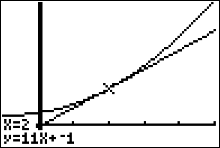
\includegraphics{./0-images/20170509-123642.png}
  \caption{This is a TI84 ScreenShot}\label{img:ti84screenshot1}
\end{figure}

Lorem ipsum dolor sit amet, consectetur adipisicing elit, sed do eiusmod tempor incididunt ut labore et dolore magna aliqua. Ut enim ad minim veniam, quis nostrud exercitation ullamco laboris nisi ut aliquip ex ea commodo consequat. Duis aute irure dolor in reprehenderit in voluptate velit esse cillum dolore eu fugiat nulla pariatur. Excepteur sint occaecat cupidatat non proident, sunt in culpa qui officia deserunt mollit anim id est laborum.

There is no need to spend any time resizing your images as this can be done by providing an option to the \verb!\includegraphics! command such as \verb![width=0.35\textwidth]!.  
\begin{figure}[h]
  \centering
  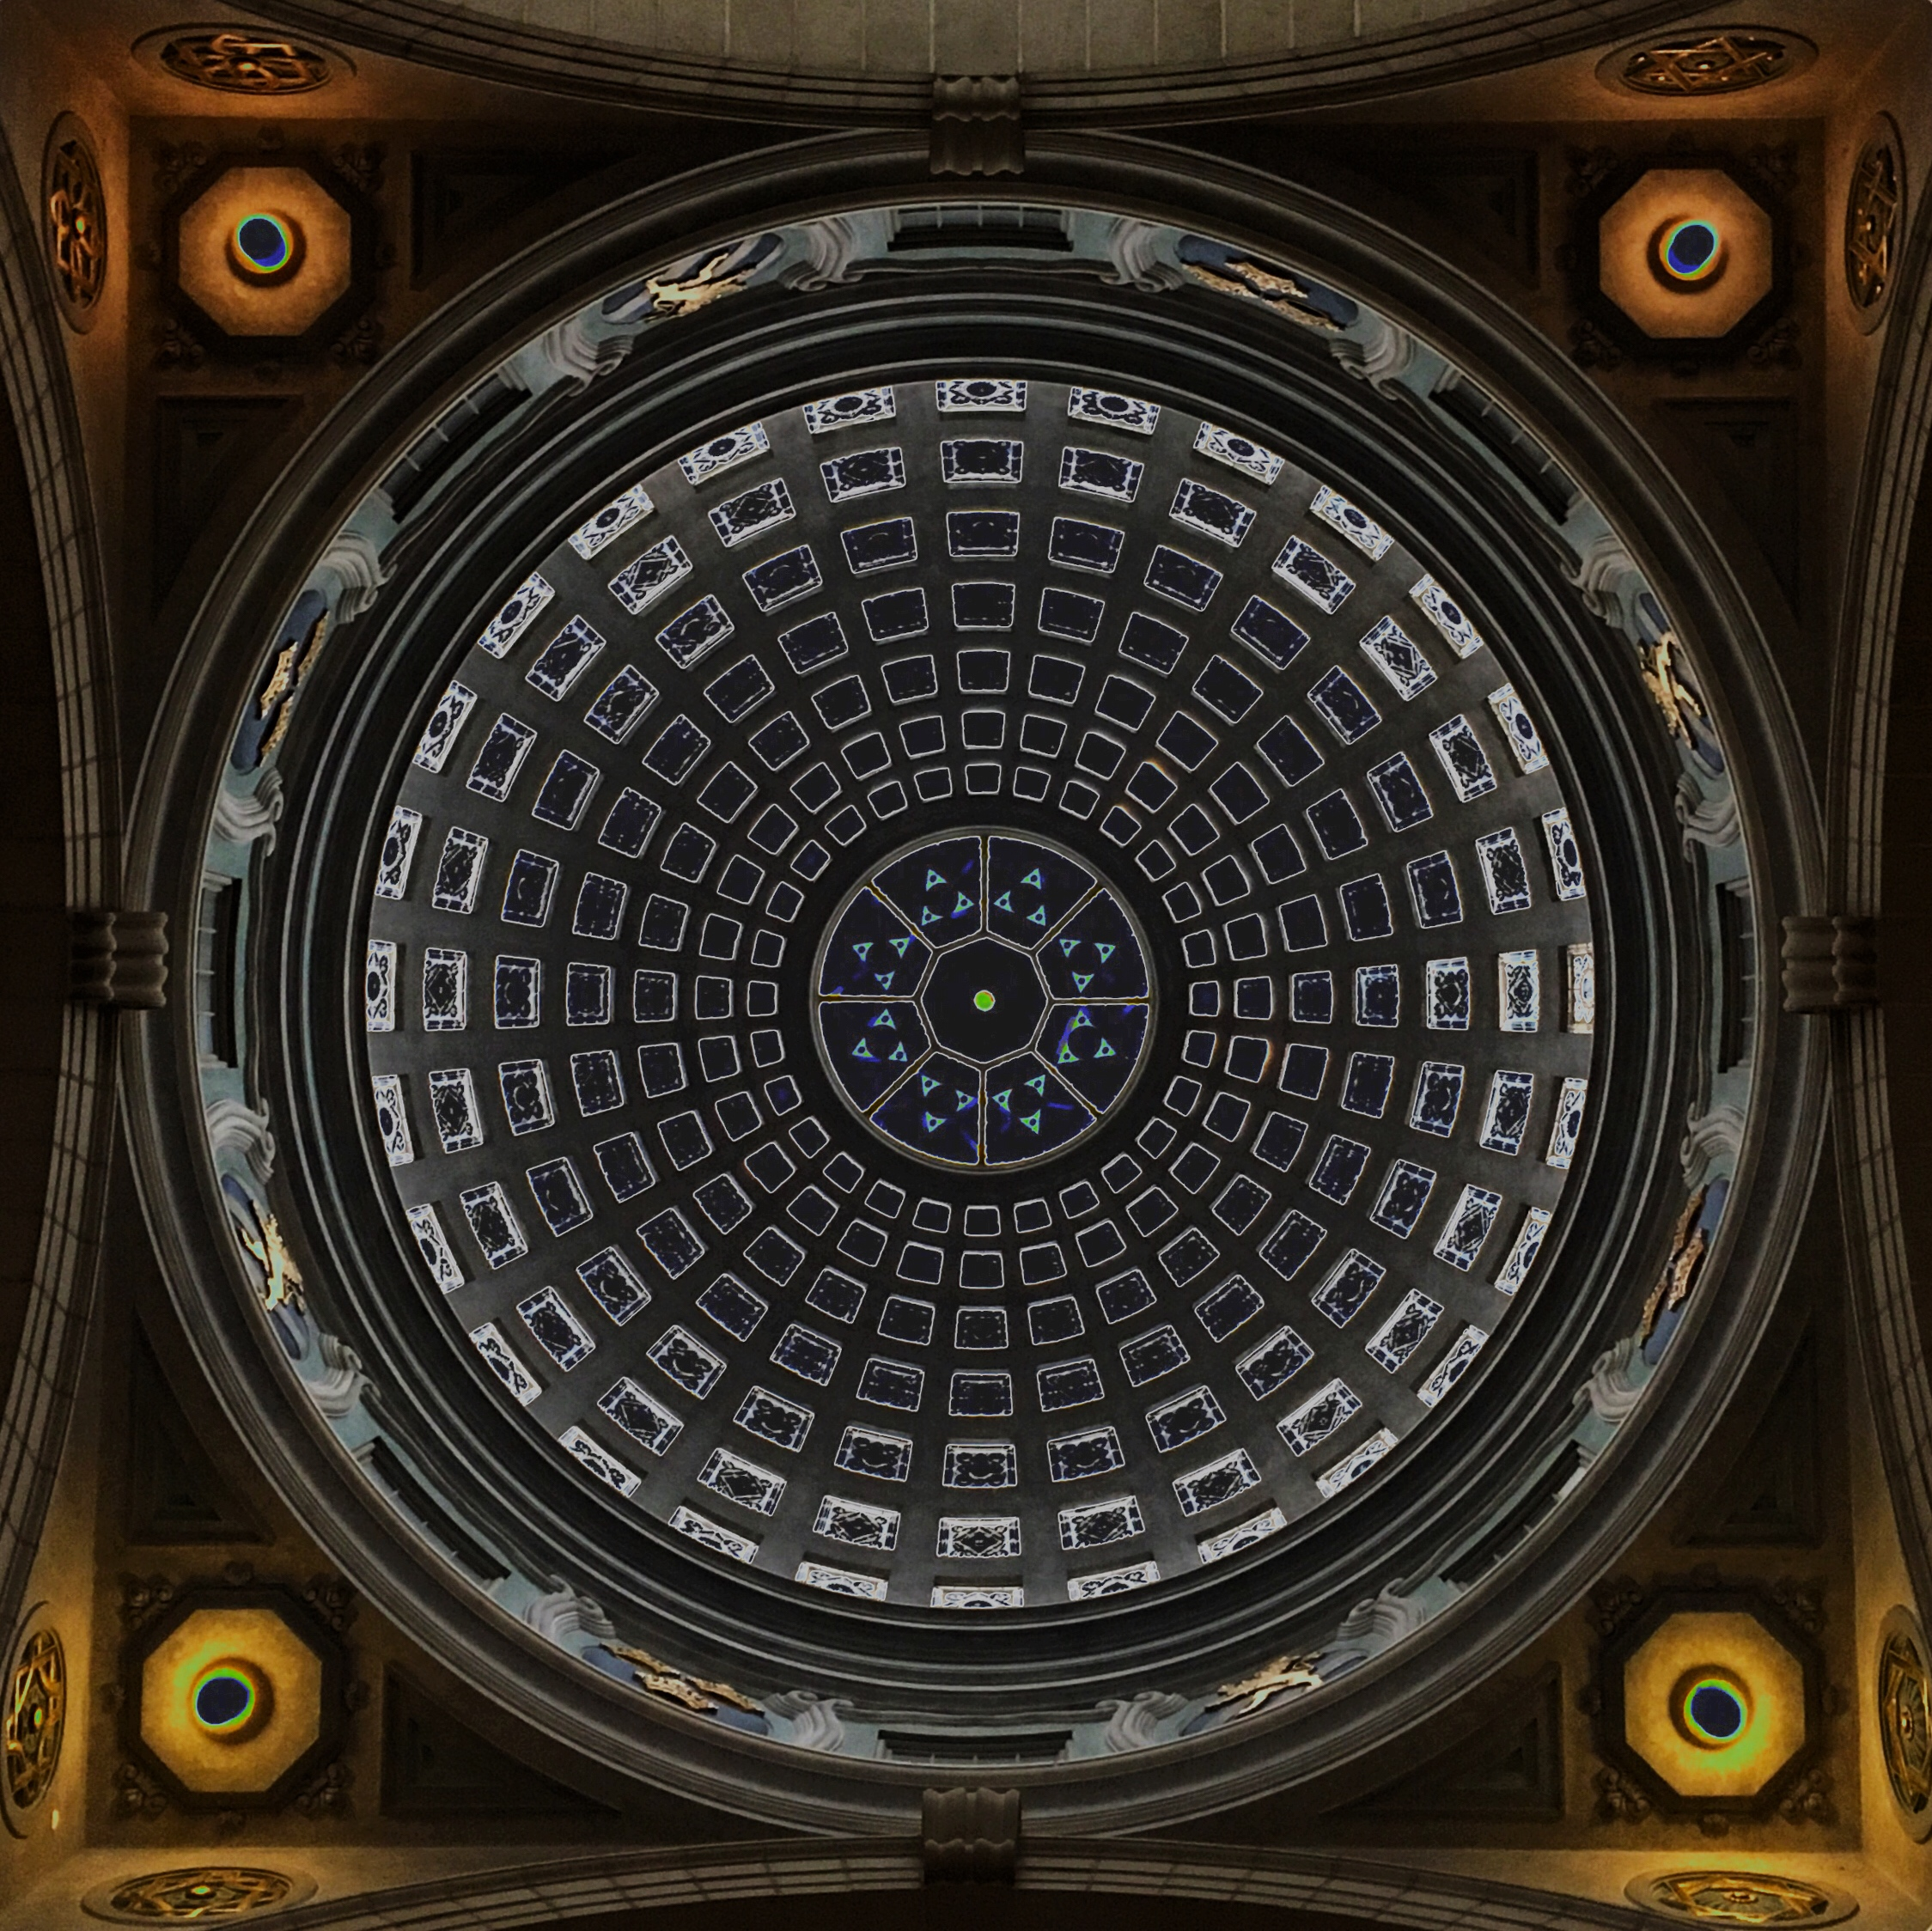
\includegraphics[width=0.35\textwidth]{./0-images/image.jpg}
  \caption{Easily resize images}
\end{figure}

Lorem ipsum dolor sit amet, consectetur adipisicing elit, sed do eiusmod tempor incididunt ut labore et dolore magna aliqua. Ut enim ad minim veniam, quis nostrud exercitation ullamco laboris nisi ut aliquip ex ea commodo consequat. Duis aute irure dolor in reprehenderit in voluptate velit esse cillum dolore eu fugiat nulla pariatur. Excepteur sint occaecat cupidatat non proident, sunt in culpa qui officia deserunt mollit anim id est laborum.\cite{mathworld:completethesquare}

If you have more than one image that you would like to group together, especially if they are the same height, then you can create a set of subfigures.  This could be good if you were maybe using some TI84 screenshots.

\begin{figure}
    \centering
    \begin{subfigure}[b]{0.3\textwidth}
        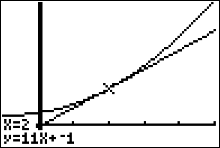
\includegraphics[width=\textwidth]{./0-images/20170509-123642.png}
        \caption{A gull}
        \label{fig:gull}
    \end{subfigure}
    ~ %add desired spacing between images, e. g. ~, \quad, \qquad, \hfill etc. 
      %(or a blank line to force the subfigure onto a new line)
    \begin{subfigure}[b]{0.3\textwidth}
        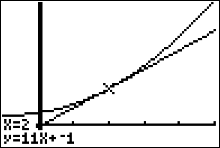
\includegraphics[width=\textwidth]{./0-images/20170509-123642.png}
        \caption{A tiger}
        \label{fig:tiger}
    \end{subfigure}
    ~ %add desired spacing between images, e. g. ~, \quad, \qquad, \hfill etc. 
    %(or a blank line to force the subfigure onto a new line)
    \begin{subfigure}[b]{0.3\textwidth}
        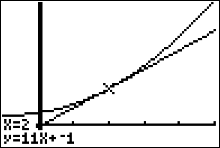
\includegraphics[width=\textwidth]{./0-images/20170509-123642.png}
        \caption{A mouse}
        \label{fig:mouse}
    \end{subfigure}
    \caption{Pictures of animals}\label{fig:animals}
\end{figure}

\subsection*{Plots}\label{subsec:plots}

You could create your plots using other software, but you might want to try using \texttt{pgfplots}.  The documentation is brilliant - so go and check it out at \url{http://pgfplots.sourceforge.net/}

\begin{figure}[ht!]
  \centering
\begin{tikzpicture}
	\begin{axis}[
            domain=-4:4,
            ymax=55,
            ymin=-80,
            %samples=100,
            axis lines =middle, xlabel=$x$, ylabel=$y$,
            every axis y label/.style={at=(current axis.above origin),anchor=south},
            every axis x label/.style={at=(current axis.right of origin),anchor=west}
          ]

          \addplot [very thick, ocBlueIX, smooth] {2*x^3-3*x^2-36*x+7};
          \addplot [very thick, ocRedIX, smooth] {12*x-6};

          \node at (axis cs:2.7,-55) {\ocBlueIX{$f(x)$}};  
          \node at (axis cs:2.8,45)  {\ocRedIX{$f''(x)$}};

		  \addplot[color=ocRedV,fill=ocRedV,only marks,mark=*] coordinates{(0.5,-11.5)};  %% closed hole
        \end{axis}
\end{tikzpicture}
\caption{Using pgfPlots for beautifully typeset graphs}
\end{figure}


%-=-=-=-=-=-=-=-=-=-=-=-=-=-=-=-=-=-=-=-=-=-=-=-=
%	YOUR IA CONTENT GOES HERE
%-=-=-=-=-=-=-=-=-=-=-=-=-=-=-=-=-=-=-=-=-=-=-=-=

\printbibliography

\end{document}